\thispagestyle{empty}

\chapter{Desarrollo de un Helicóptero Semilla a Partir de un Helicóptero Base}

\spacing{1.5}

Comenzar el desarrollo del vehículo desde el principio supondría un esfuerzo y trabajo innecesarios, por lo que lo ideal es la obtención de un helicóptero semilla, un modelo que sirva de primera aproximación sobre el que trabajar y hacer modificaciones. Este helicóptero semilla se obtendrá mediante una adimensionalización de las características de un vehículo real y posterior dimensionalización empleando los parámetros que deba poseer el nuevo vehículo.

Todo este proceso se describirá a lo largo de este capítulo de manera que una vez terminado se tengan los datos necesarios para poder comenzar a realizar simulaciones de vuelo.

\section{Descripción Helicóptero Base}

El primer paso es elegir un modelo que sirva de base para nuestros cálculos y permita obtener un primer diseño lo mas cercano posible al resultado que se desee. El requisito más importante que debe cumplir esta aeronave será que resulte semejante al diseño que se busca, de manera que pueda reescalarse según las necesidades. Para este proyecto se ha escogido el Bölkow Bo 105, un helicóptero utilitario monorrotor, cuyas características se exponen a continuación. Cabe indicar que todos los parámetros definidos conformarán una estructura en MATLAB que se empleará en los cálculos.

\subsection{Rotor Principal del Bo 105}

Los parámetros necesarios para definir el rotor principal de un helicóptero incluyen datos geométricos, aerodinámicos y de inercia. Los correspondientes al Bo 105 se encuentran recogidos en la tabla \ref{RPBo}.
Para simplificar los cálculos, la pala se modeliza como sólido rígido, unida al rotor por un muelle de constante $k_\beta$.
Además el tensor de inercia de la pala se ha modelizado de la siguiente manera:

\begin{equation}
[I_B]=\left[	
\begin{array}{ccc}
I_\beta & 0 & 0\\
0 & I_\theta & 0\\
0 & 0 & I_\zeta
\end{array}
\right]
\end{equation}

\begin{table}[]
	\centering
	\begin{tabular}{|>{\columncolor{Gray}}c|c|}
		\hline
		Radio de las palas ($R$) & 4.91 m \\ \hline
		Excentricidad ($e$) & 0 m \\ \hline
		Número de palas ($b$) & 4 \\ \hline
		Torsión lineal de los perfiles ($\theta_1$) & -0.14 \\ \hline
		Pendiente de la curva de sustentación ($\alpha$) & 6.113 rad$^{-1}$ \\ \hline
		\cellcolor{Gray} & 0.0074 \\ \cline{2-2} 
		\cellcolor{Gray} & 0.00961 rad$^{-1}$ \\ \cline{2-2} 
		\multirow{-3}{*}{\cellcolor{Gray}Parámetros de la polar ($\delta_0$, $\delta_1$, $\delta_2$)} & 0.29395 rad$^{-2}$ \\ \hline
		Velocidad de giro del rotor ($\Omega$) & 44.4 rad/s \\ \hline
		Cuerda del perfil ($c$) & 6.113 m \\ \hline
		Momento de inercia de la pala en batimiento ($I_\beta$) & 231.7 kgm$^2$ \\ \hline
		Momento de inercia de la pala en paso ($I_\theta$) & 7 kgm$^2$ \\ \hline
		Momento de inercia de la pala en arrastre ($I_\zeta$) & 238.7 kgm$^2$ \\ \hline
		Posición del centro de gravedad de la pala ($x_{GB}$) & 2.445 m \\ \hline
		Masa de la pala ($m_b$) & 40.2 kg \\ \hline
		Rigidez en batimiento ($k_\beta$) & 113330 Nm/rad \\ \hline
	\end{tabular}
	\caption{Valores de diferentes parámetros del rotor principal de la aeronave Bölkow Bo 105.}
	\label{RPBo}
\end{table}

\subsection{Rotor Antipar del Bo 105}

Los parámetros necesarios para definir el rotor antipar de un helicóptero son los mismos que definen el rotor principal, y pueden encontrarse en la tabla \ref{RaBo}.
Las mismas consideraciones aplicadas al rotor principal a la hora de modelizarlo se aplican al rotor antipar. Además se considera que la masa de la pala se encuentra uniformemente distribuida a lo largo de la envergadura de la misma y que la unión resulta infinitamente rígida en batimiento.
\begin{table}[htbp]
	\centering
	\begin{tabular}{|>{\columncolor{Gray}}c|c|}
		\hline
		Radio de las palas ($R$) & 0.95 m \\ \hline
		Excentricidad ($e$) & 0 m \\ \hline
		Número de palas ($b$) & 2 \\ \hline
		Torsión lineal de los perfiles ($\theta_1$) & \cellcolor[rgb]{ 1,  1,  1}0 \\ \hline
		Pendiente de la curva de sustentación ($\alpha$) & 5.7 rad$^{-1}$ \\ \hline
		\cellcolor{Gray} & 0.008 \\ \cline{2-2}
		\cellcolor{Gray} & 0.0096 rad$^{-1}$ \\ \cline{2-2}
		\multirow{-3}{*}{\cellcolor{Gray}Parámetros de la polar ($\delta_0$, $\delta_1$, $\delta_2$)} & 0.294 rad$^{-2}$ \\ \hline
		Velocidad de giro del rotor ($\Omega$) & \cellcolor[rgb]{ 1,  1,  1}232.4779 rad/s \\ \hline
		Cuerda del perfil ($c$) & \cellcolor[rgb]{ 1,  1,  1}0.18 m \\ \hline
		Momento de inercia de la pala en batimiento ($I_\beta$) & 1.805 kgm$^2$ \\ \hline
		Momento de inercia de la pala en paso ($I_\theta$) & 0.0648 kgm$^2$ \\ \hline
		Momento de inercia de la pala en arrastre ($I_\zeta$) & 1.8698 kgm$^2$ \\ \hline
		Posición del centro de gravedad de la pala ($X_{GB}$) & 0.475 m \\ \hline
		Masa de la pala ($m_b$) & 6 $kg$ \\ \hline
		\cellcolor{Gray}Rigidez en batimiento ($I_\beta$) & $10^{100}$ Nm/rad \\ \hline
	\end{tabular}%
	\caption{Valores de diferentes parámetros del rotor antipar de la aeronave Bölkow Bo 105.}
	\label{RaBo}
\end{table}%

Además de esta información de los rotores, es necesaria una modelización de las pérdidas en las trasmisiones:

\begin{itemize}
	\item $\eta_{Trp}=0.12$
	\item $\eta_{Tra}=0.07$
\end{itemize}

\subsection{Fuselaje del Bo 105}

Los parámetros más relevantes del fuselaje serán aquellos necesarios para la adimensionalización de las fuerzas y momentos sobre el mismo, es decir, las superficies de referencia y la longitud del fuselaje $l_f$. Estos datos se recogen en la tabla \ref{FBo}.

\begin{table}[htbp]
	\centering
	\begin{tabular}{|>{\columncolor{Gray}}c|c|}
		\hline
		\cellcolor{Gray}Longitud del fuselaje ($l_f$) & \cellcolor[rgb]{ 1,  1,  1}8.56 m \\ \hline
		\cellcolor{Gray}Superficie en planta del fuselaje ($S_p$)& \cellcolor[rgb]{ 1,  1,  1}7.5 m$^2$ \\ \hline
		\cellcolor{Gray}Superficie lateral del fuselaje ($S_l$) & \cellcolor[rgb]{ 1,  1,  1}8.3 m$^2$ \\ \hline
		\cellcolor{Gray}Factor de interferencia del rotor principal sobre el fuselaje ($k_f$) & \cellcolor[rgb]{ 1,  1,  1}1 \\ \hline
		\end{tabular}%
	\caption{Valores de los parámetros del fuselaje de la aeronave Bölkow Bo 105.}
	\label{FBo}
\end{table}%

La formulación de los coeficientes de fuerzas y momentos es la siguiente:

\begin{equation}
K_x^f=\frac{-580.6-454\alpha_f+6.2\alpha_f^2+4648.9\alpha_f^3}{\frac{1}{2}\rho V_f^2S_p}
\end{equation}
\begin{equation}
K_y^f=\frac{-6.9-2399\beta_f-1.7\beta_f^2+12.7\beta_f^3}{\frac{1}{2}\rho V_f^2S_l}
\end{equation}
\begin{equation}
K_z^f=\frac{-51.1-1202\alpha_f+1515.7\alpha_f^2-64.2\alpha_f^3}{\frac{1}{2}\rho V_f^2S_p}
\end{equation}
\begin{equation}
K_{M_x}^f=0
\end{equation}
\begin{equation}
K_{M_y}^f=\frac{-1191.8+12752\alpha_f+8201.3\alpha_f^2-5796.7\alpha_f^3}{\frac{1}{2}\rho V_f^2S_pl_f}
\end{equation}
\begin{equation}
K_{M_z}^f=\frac{-10028\beta_f}{\frac{1}{2}\rho V_f^2S_ll_f}
\end{equation}


\subsection{Estabilizadores del Bo 105}

Los parámetros que definen a los estabilizadores vertical y horizontal se encuentran recogidos en la tabla \ref{EBo}. Se puede observar que son datos similares a los que tendrían las alas de un avión, obviando los controles e hipersustentadores, ya que aerodinámicamente funcionan de la misma manera, solo que las fuerzas que generan ayudan a aumentar la estabilidad de la aeronave o reducir la potencia del rotor antipar, entre otras funciones.
Se ha considerado que no tienen estrechamiento, son rectos y están formados por un único perfil, motivo por el que el número de parámetros es tan reducido.
En el caso del estabilizador horizontal, este se divide en dos partes, por lo que la superficie corresponde únicamente a la mitad del mismo.

\begin{table}[htbp]
	\centering
	\begin{tabular}{|>{\columncolor{Gray}}c|c|}
		\hline
		\cellcolor{Gray}Cuerda del estabilizador vertical ($c_{ev}$) & \cellcolor[rgb]{ 1,  1,  1}0.3 m \\ \hline
		\cellcolor{Gray}Superficie del estabilizador vertical ($S_{ev}$)& \cellcolor[rgb]{ 1,  1,  1}0.805 m$^2$ \\ \hline
		\cellcolor{Gray}Ángulo de calado del estabilizador vertical ($\theta_{ev}$) & \cellcolor[rgb]{ 1,  1,  1}0.0812 rad \\ \hline
		\cellcolor{Gray}Cuerda del estabilizador horizontal ($c_{ev}$) & \cellcolor[rgb]{ 1,  1,  1}0.4 m \\ \hline
		\cellcolor{Gray}Superficie del estabilizador horizontal/2 ($S_{ev}$)& \cellcolor[rgb]{ 1,  1,  1}0.4015 m$^2$ \\ \hline
		\cellcolor{Gray}Ángulo de calado del estabilizador horizontal ($\theta_{ev}$) & \cellcolor[rgb]{ 1,  1,  1}0.0698 rad \\ \hline
	\end{tabular}%
	\caption{Valores de diferentes parámetros de los estabilizadores vertical y horizontal de la aeronave Bölkow Bo 105. La superficie del estabilizador horizontal corresponde a la mitad ya que el mismo esta dividido en 2 partes.}
	\label{EBo}
\end{table}%

\subsection{Geometría del Bo 105}

Es importante conocer las características geométricas del modelo ya que en base a ella se calcularán, entre otros parámetros, los momentos sobre la aeronave, muy importantes para calcular el equilibrado de la misma.
Dichas características se recogen en la tabla \ref{GeBo} y se han representado en la figura \ref{GeBodraw} una esquematización de las mismas para ayudar a su comprensión.

\begin{figure}
	\centering
	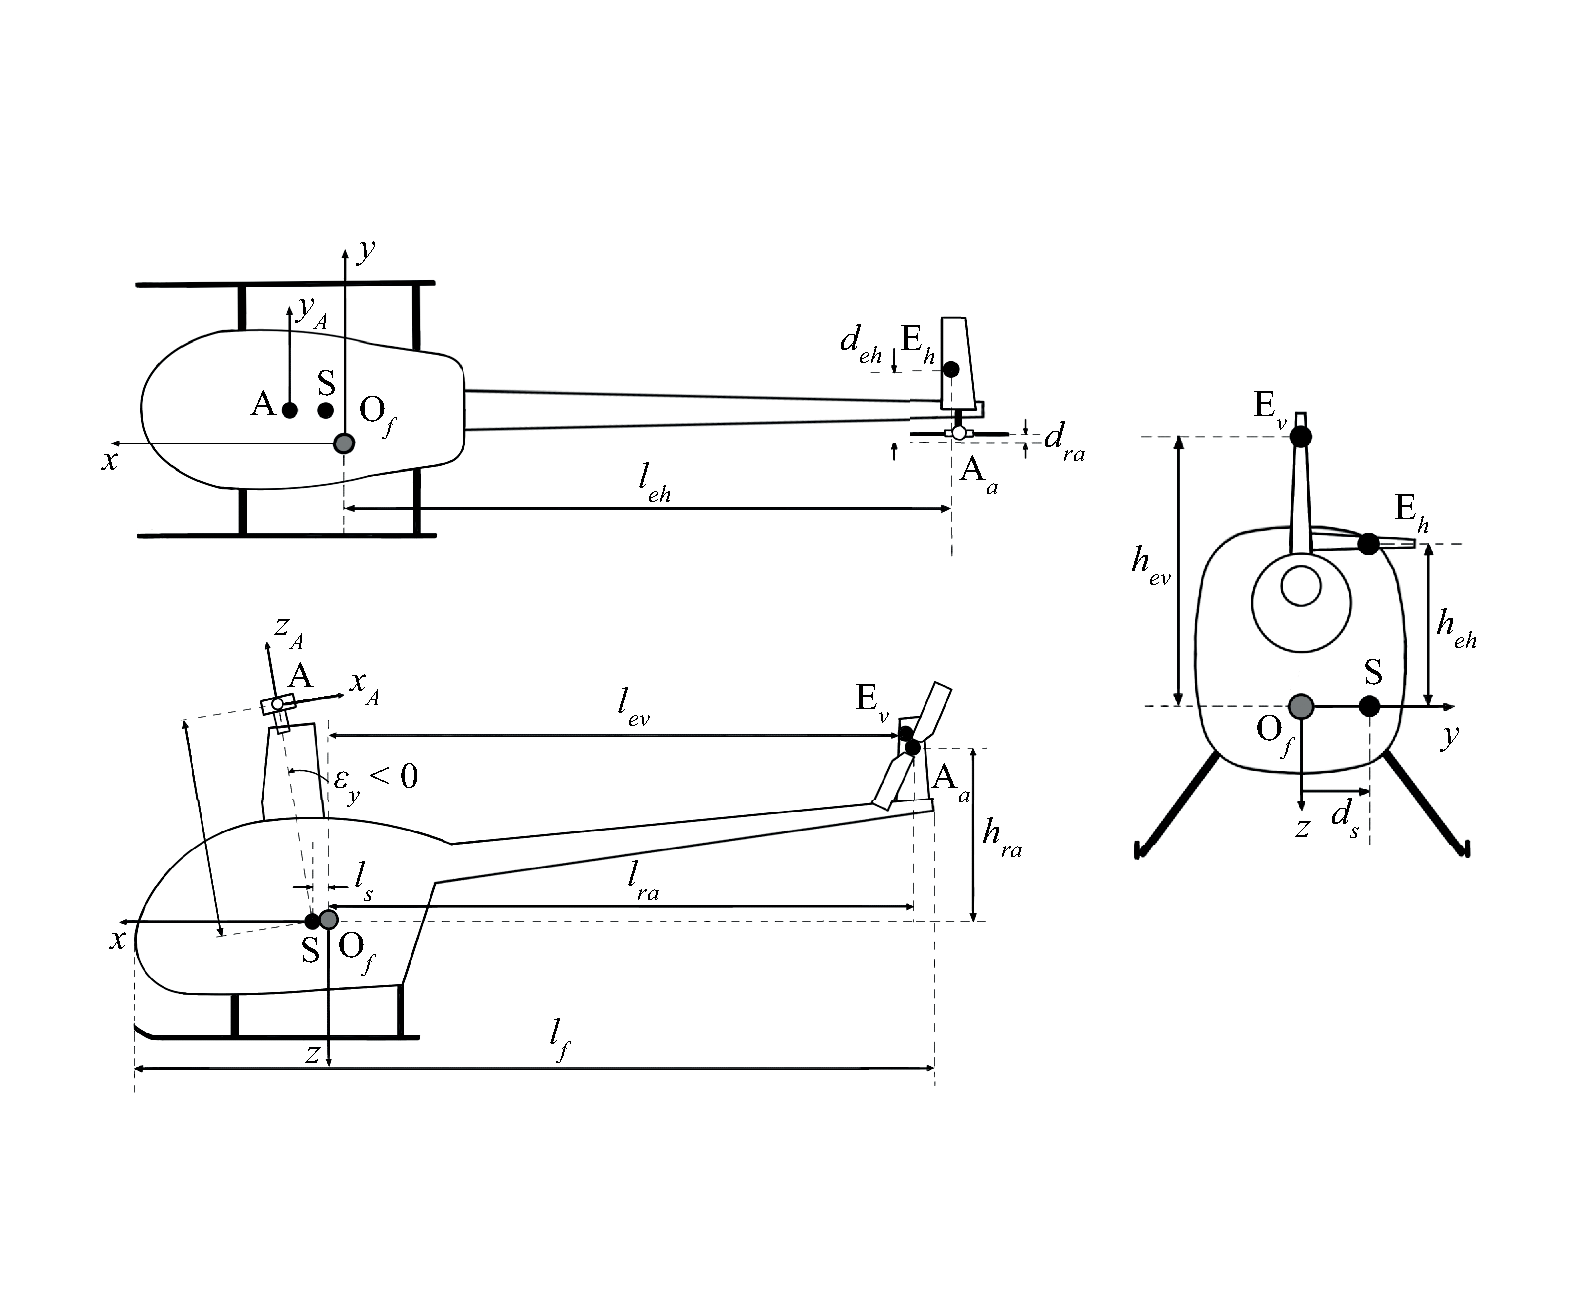
\includegraphics[width=120mm]{imagenes/geometria}
	\caption{Esquema de las medidas indicadas en la tabla \ref{GeBo} sobre las distintas vistas de un helicóptero genérico.}
	\label{GeBodraw}
\end{figure}

\begin{table}[htbp]
	\centering
	\begin{tabular}{|>{\columncolor{Gray}}c|c|}
		\hline
		\cellcolor{Gray}Posición longitudinal del centro de masas respecto a $O_f$ ($x_{CG}$) & 0.1577 m \\ \hline
		\cellcolor{Gray}Posición lateral del centro de masas respecto a $O_f$ ($y_{CG}$) & 0 m \\ \hline
		\cellcolor{Gray}Posición vertical del centro de masas respecto a $O_f$ ($z_{CG}$) & 0 m \\ \hline
		\cellcolor{Gray}Inclinación del eje del árbol respecto al plano $xz$ ($\varepsilon_x$) & 0 rad \\ \hline
		\cellcolor{Gray}Inclinación del eje del árbol respecto al plano $yz$ ($\varepsilon_y$) & -0.523 rad \\ \hline
		\cellcolor{Gray}Componente $x$ del vector $\boldsymbol{O_fS}$ ($l_s$) & 0 m \\ \hline
		\cellcolor{Gray}Componente $y$ del vector $\boldsymbol{O_fS}$ ($d_s$) & 0 m \\ \hline
		\cellcolor{Gray}Longitud del árbol, desde $S$ hasta $A$ ($h$) & 1.48 m \\ \hline
		\cellcolor{Gray}Inclinación del rotor antipar ($\theta_{ra}$) & 0 rad \\ \hline
		\cellcolor{Gray}Componente $x$ del vector $\boldsymbol{O_fA_a}$ ($l_{ra}$) & -5.9226 m \\ \hline
		\cellcolor{Gray}Componente $y$ del vector $\boldsymbol{O_fA_a}$ ($d_{ra}$) & -0.3 m \\ \hline
		\cellcolor{Gray}Componente $z$ del vector $\boldsymbol{O_fA_a}$ ($h_{ra}$) & -1.6426 m \\ \hline
		\cellcolor{Gray}Ángulo de orientación del estabilizador vertical ($\gamma_{ev}$) & $\pi$/2 rad \\ \hline
		\cellcolor{Gray}Componente $x$ del vector $\boldsymbol{O_fE_v}$ ($l_{ev}$) & -5.3386 m \\ \hline
		\cellcolor{Gray}Componente $y$ del vector $\boldsymbol{O_fE_v}$ ($d_{ev}$) & 0 m \\ \hline
		\cellcolor{Gray}Componente $z$ del vector $\boldsymbol{O_fE_v}$ ($h_{ev}$) & -0.86 m \\ \hline
		\cellcolor{Gray}Ángulo de orientación del estabilizador horizontal (dcha.) ($\gamma_{eh,d}$) & 0 rad \\ \hline
		\cellcolor{Gray}Componente $x$ del vector $\boldsymbol{O_fE_h}$ parte dcha. ($l_{eh,d}$) & -4.4826 m \\ \hline
		\cellcolor{Gray}Componente $y$ del vector $\boldsymbol{O_fE_h}$ parte dcha. ($d_{eh,d}$) & 0.969 m \\ \hline
		\cellcolor{Gray}Componente $z$ del vector $\boldsymbol{O_fE_h}$ parte dcha. ($h_{eh,d}$) & 0 m \\ \hline
		\cellcolor{Gray}Ángulo de orientación del estabilizador horizontal (izqda.) ($\gamma_{eh,i}$) & 0 rad \\ \hline
		\cellcolor{Gray}Componente $x$ del vector $\boldsymbol{O_fE_h}$ parte izqda. ($l_{eh,i}$) & -4.4826 m \\ \hline
		\cellcolor{Gray}Componente $y$ del vector $\boldsymbol{O_fE_h}$ parte izqda. ($d_{eh,i}$) & -0.969 m \\ \hline
		\cellcolor{Gray}Componente $z$ del vector $\boldsymbol{O_fE_h}$ parte izqda. ($h_{eh,i}$) & 0 m \\ \hline
	\end{tabular}%
	\caption{Valores de diferentes parámetros geométricos de la aeronave Bölkow Bo 105.}
	\label{GeBo}
\end{table}%

\subsection{Inercia del Bo 105}

Para finalizar con la descripción del modelo del helicóptero, la tabla \ref{InBo} refleja los datos acerca de la inercia del mismo.

\begin{table}[htbp]
	\centering
	\begin{tabular}{|>{\columncolor{Gray}}c|c|}
		\hline
		\cellcolor{Gray}Peso del helicóptero ($W$) & \cellcolor[rgb]{ 1,  1,  1}21560 N \\ \hline
		\cellcolor{Gray}Momento de inercia del eje $x$ ($I_{x}$) & \cellcolor[rgb]{ 1,  1,  1}1433 kg$\cdot$m$^2$ \\ \hline
		\cellcolor{Gray}Momento de inercia del eje $y$ ($I_{y}$) & \cellcolor[rgb]{ 1,  1,  1}4973 kg$\cdot$m$^2$ \\ \hline
		\cellcolor{Gray}Momento de inercia del eje $z$ ($I_{z}$) & \cellcolor[rgb]{ 1,  1,  1}4099 kg$\cdot$m$^2$ \\ \hline
		\cellcolor{Gray}Producto de inercia $xy$ ($I_{xy}$)& \cellcolor[rgb]{ 1,  1,  1}0 kg$\cdot$m$^2$ \\ \hline
		\cellcolor{Gray}Producto de inercia $xz$ ($I_{xz}$)& \cellcolor[rgb]{ 1,  1,  1}660 kg$\cdot$m$^2$ \\ \hline
		\cellcolor{Gray}Producto de inercia $yz$ ($I_{yz}$)& \cellcolor[rgb]{ 1,  1,  1}0 kg$\cdot$m$^2$ \\ \hline
	\end{tabular}%
	\caption{Valores de inercia de la aeronave Bölkow Bo 105.}
	\label{InBo}
\end{table}%

Con este modelo y los parámetros de diseño calculado estadísticamente se generará un modelo inicial que se empleará en las simulaciones para comprobar su desempeño y optimizarlo según las necesidades.

\section{Adimensionalización del Modelo}

Una vez esta definido el helicóptero base, es necesario realizar una adimensionalización del modelo para poder obtener luego un modelo válido para el diseño requerido.

En \citet{Cuerva} se habla de dos posibles adimensionalizaciones en el ámbito de los helicópteros, cada cual con una velocidad característica:

\begin{itemize}
	\item Primera forma adimensional: se emplea la velocidad inducida dada por la teoría de la cantidad de movimiento en vuelo a punto fijo, $v_{i0}$.
	\item Segunda forma adimensional: se emplea la velocidad en punta de pala, $\Omega R$, con $\Omega$ la velocidad de giro del rotor y $R$ el radio del mismo. Usar esta velocidad como velocidad de referencia permite definir magnitudes características de fuerza, par y potencia.
\end{itemize}

Debido a la existencia de parámetros de fuerza, par y potencia en el modelo del Bölkow Bo 105, resulta conveniente emplear la segunda forma adimensional, lo que define las siguientes magnitudes de fuerza, par y potencia:

\begin{itemize}
	\item Tracción unitaria: $T_u=\rho S(\Omega R)^2$, donde $S=\pi R^2$
	\item Par unitario: $Q_u=\rho SR(\Omega R)^2$
	\item Potencia unitaria: $P_u=\rho S(\Omega R)^3$
\end{itemize}

Estas magnitudes permiten a su vez definir los coeficientes de tracción, $C_T=\frac{T}{T_u}$, y de potencia o par, $C_Q=C_P=\frac{Q}{Q_u}=\frac{P}{P_u}$.

Una vez definida la formulación adimensional a usar, solo resta adimensionalizar cada una de las estructuras definidas en el apartado anterior.

\subsection{Rotores Principal y Antipar}

Adimensionalizar los parámetros correspondientes a ambos rotores requiere el uso de magnitudes características de longitud y velocidad, que serán el radio del rotor y la velocidad en punta de pala, pero además el modelo computacional de \emph{HEROES} requerirá de los parámetros atmosféricos a nivel del mar (H=0) de gravedad, $g$, densidad, $\rho$, viscosidad dinámica del fluido y velocidad del sonido.

Al adimensionalizar la estructura del helicóptero base se obtendrán para cada rotor estructuras con los siguientes parámetros:
\singlespacing
\begin{multicols}{2}
	\begin{itemize}
		\item Número de palas: $b$
		\item Solidez del rotor: $\sigma=\frac{c\cdot b}{\pi\cdot R}$
		\item Parámetros de la polar: $\delta_0$, $delta_1$ y $\delta_2$
		\item Coeficiente de sustentación de los perfiles: $c_l$
		\item Torsión lineal de los perfiles: $\theta_1$
		\item Excentricidad adimensional: $e/R$
		\item $\varepsilon_R=\frac{m_b\cdot R\cdot x_{GB}}{I_\beta}$
		\item "Gravedad adimensional"$=\frac{g}{\Omega^2R}$
		\item Rigidez en batimiento adimensional: $K_\beta=\frac{k_\beta}{\rho \pi R^2(\Omega R)^2R}$
		\item Frecuencia natural adimensional no amortiguada en batimiento: $\lambda_\beta=1+\frac{x_{GB}\cdot m_b\cdot e}{I_\beta}+\frac{k_\beta}{I_\beta\cdot\Omega^2}$
		\item Número de Lock: $\gamma=\frac{\rho c_0cR^4}{I_\beta}$
		\item Número de rigidez: $S_\beta=\frac{8(\lambda_\beta^2-1)}{\gamma}$
		\item Relación adimensional $I_\theta/I_\beta$
		\item Relación adimensional $I_\zeta/I_\beta$
		\item Posición adimensional del centro de gravedad de la pala: $X_{GB}=x_{GB}/R$
		\item Parámetro $\mu_p=\frac{m_b}{\rho\pi R^3}$
		\item Número de Reynolds: $Re$
		\item Número de Mach: $M=\frac{\Omega R}{v_{sound}}$
		\end{itemize}
\end{multicols}
\spacing{1.5}
Además de estos parámetros, en la estructura del helicóptero adimensional (la correspondiente al helicóptero completo, no a la de los rotores) aparecerán también los siguientes parámetros:
\singlespacing
\begin{multicols}{2}
	\begin{itemize}
		\item Relación de velocidades angulares: $\frac{\Omega_a}{\Omega}$
		\item Relación de velocidades: $\frac{\Omega_aR_a}{\Omega R}$
		\item Relación de fuerzas $\frac{(\Omega_aR_a)^2R_a^2}{(\Omega R)^2R^3}$
		\item Relación de momentos $\frac{(\Omega_aR_a)^2R_a^2}{(\Omega R)^2R^3}$
	\end{itemize}
\end{multicols}
\spacing{1.5}
\subsection{Fuselaje}

Al estar la estructura del fuselaje compuesta únicamente por características físicas y coeficientes aerodinámicos, solo es necesario definir las adimensionalizaciones para los primeros, pues los segundos ya lo están. Dichas adimensionalizaciones quedarían de la siguiente forma:

\singlespacing
\begin{multicols}{2}
	\begin{itemize}
		\item Longitud del fuselaje: $l_f/R$
		\item Superficie en planta del fuselaje: $\frac{S_s}{\pi R^2}$
		\item Superficie lateral del fuselaje: $\frac{S_l}{\pi R^2}$
	\end{itemize}
\end{multicols}
\spacing{1.5}

Aunque no es un coeficiente aerodinámico, el factor de interferencia del rotor principal con el fuselaje, $k_f$, ya es adimensional por lo que no es necesario trabajarlo.

\subsection{Estabilizadores Vertical y Horizontal}

El caso de los estabilizadores es similar al del fuselaje, únicamente será necesario indicar las adimensionalizaciones de las características físicas ya que el resto son parámetros adimensionales, los cuales quedaría de la siguiente forma:

\singlespacing
\begin{multicols}{2}
	\begin{itemize}
		\item Estabilizador vertical
		\subitem Cuerda del perfil adimensional: $c_{ev}/R$
		\subitem Superficie adimensional: $\frac{S_{ev}}{\pi R^2}$
		\item Estabilizador horizontal
		\subitem Cuerda del perfil adimensional: $c_{eh}/R$
		\subitem Superficie adimensional: $\frac{S_{eh}}{\pi R^2}$
	\end{itemize}
\end{multicols}
\spacing{1.5}

\subsection{Geometría e Inercia del Helicóptero}

En lo que respecta a la geometría, la adimensionalización resulta tan simple como emplear el radio del rotor $R$ para todos los parámetros.

Por otro lado, al adimensionalizar los parámetros de inercia quedarán como se indica a continuación:

\singlespacing
\begin{multicols}{2}
	\begin{itemize}
		\item Coeficiente de peso: $C_w=\frac{W}{T_u}$
		\item Parámetro adimensional $\gamma_x=\frac{\rho\pi R^5}{I_x}$
		\item Parámetro adimensional $\gamma_y=\frac{\rho\pi R^5}{I_y}$
		\item Parámetro adimensional $\gamma_z=\frac{\rho\pi R^5}{I_z}$
		\item Relación adimensional $\frac{I_x}{I_y}$
		\item Relación adimensional $\frac{I_z}{I_y}$
		\item Relación adimensional $\frac{I_{xy}}{I_y}$
		\item Relación adimensional $\frac{I_{xz}}{I_y}$
		\item Relación adimensional $\frac{I_{yz}}{I_y}$
	\end{itemize}
\end{multicols}
\spacing{1.5}

Con todos estos datos y los parámetros de diseño radio del rotor, velocidad de giro de rotor, numero de palas del rotor principal y antipar y peso del nuevo helicóptero, se puede obtener un modelo completo para el nuevo diseño.

\section{Limitaciones a la Velocidad de Giro del Rotor Principal}

Aunque se han calculado estadísticamente los parámetros que definen en una primera aproximación el vehículo a diseñar, debido a la falta de datos de helicópteros existentes similares y a la dispersión de los pocos de los que se dispone suficiente información, es probable que el modelo no resulte realista y no pueda llegar a funcionar correctamente en una situación de vuelo fuera de la simulación. El parámetro del que menos información se dispone es de la velocidad de giro de los rotores de los modelos de las base de datos, por lo que conviene encontrar un valor que pueda resultar mejor. Para ello se ha empleado un concepto físico importante como es el Mach crítico $M_{crit}$ en la punta de pala.

La limitación en la velocidad de giro del rotor viene dada por la aparición de efectos supersónicos en las puntas de las palas del mismo. Estos efectos, como puedan ser ondas de choque, empeoran el comportamiento de las palas, pueden hacerlas entrar en pérdida e incluso provocar daños estructurales debido a cargas elevadas.
Por esto es común establecer un límite conocido como $M_{crit}$ basado en la velocidad $\Omega R$, es decir, la velocidad de avance de las puntas de las palas. Este límite suele ser del orden de 0,4 para vuelo estacionario y 0,8 para vuelo en avance. 
Para poder dar un valor lo más óptimo posible, se ha realizado una simulación de vuelo estacionario de un vehículo con las características obtenidas estadísticamente, a excepción de la velocidad de giro del rotor principal y del radio del mismo, que se han variado para poder obtener el mejor valor posible de estos parámetros.


\begin{figure}
	\centering
	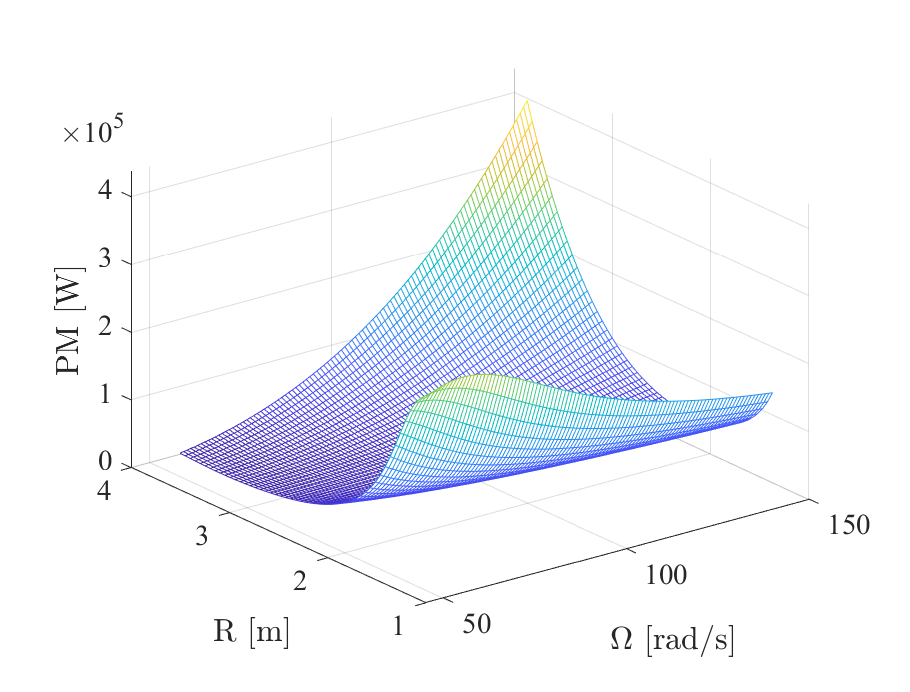
\includegraphics[width=90mm]{graficos/3d3d}
	\caption{Consumo de Potencia de la aeronave en función de la velocidad de giro del rotor y el radio del mismo.}
	\label{ORP}
\end{figure}
\begin{figure}
	\centering
	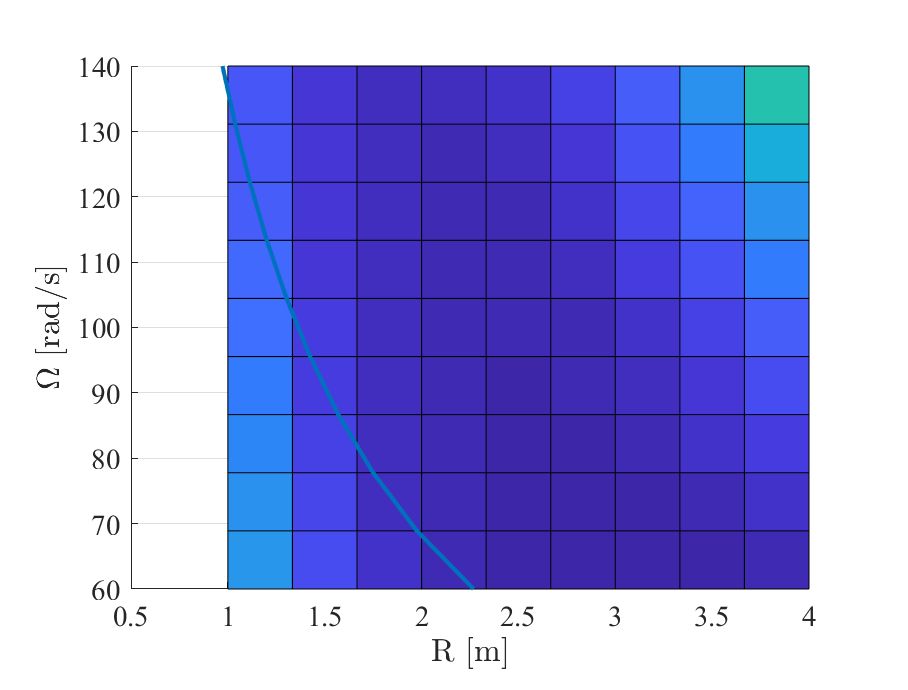
\includegraphics[width=90mm]{graficos/3d2d}
	\caption{Consumo de Potencia de la aeronave en función de la velocidad de giro del rotor y el radio del mismo junto a la línea de las potencias mínimas para cada configuración concreta de $\Omega$ y la limitación de $\Omega$ a causa del $M_{crit}$ (0,4).}
	\label{ORPM}
\end{figure}

La gráfica \ref{ORP} representa la superficie que da un valor de potencia de la aeronave para cada $\Omega$ y $R$ del rotor. Con esto es posible observar los valores mínimos de potencia, lo que nos permite elegir unos valores de $\Omega$ y $R$ que optimicen la potencia necesaria.
Sin embargo, al añadir la limitación del $M_{crit}$ las opciones de configuración disponibles se ven reducidas a aquellas que la cumplan. La gráfica \ref{ORPM} representa la superficie de la gráfica \ref{ORP} sobre el plano $\Omega R$ y encima la anterior limitación junto con una línea que representa las potencias mínimas absolutas para cada configuración de $\Omega$. Aunque estas líneas no se crucen, para los valores más bajos de $\Omega$ se encuentran suficientemente cerca como para pensar que las potencias necesarias son lo suficientemente bajas.
Se observa claramente que los valores de potencia necesaria se reducen con $\Omega$ y con el aumento de radio, por lo que en primera instancia el menor valor dado, quedando automáticamente definido el radio del rotor.

\begin{itemize}
	\item Velocidad de giro del rotor principal $\Omega$ = 45 $rad/s$
	\item Radio del rotor principal $R$ = 3.0248 $m$
\end{itemize}

\section{Obtención del modelo del helicóptero \emph{DroneHE}}

El objetivo es obtener un modelo de helicóptero lo más próximo posible al diseño final sobre el que se puedan realizar unas primeras simulaciones de vuelo para comprobar si es válido y, en caso contrario, modificar el diseño para alcanzar unos resultados mejores. Su obtención se consigue empleando la herramienta \emph{HEROES}, que primero adimensionalizará el helicóptero base ya definido en el capítulo como se ha visto, para después dimensionar un nuevo modelo, al que llamaremos \emph{DroneHE}, usando los parámetros que hemos obtenido. Los resultados se recogen en las tablas \ref{RPHS}, \ref{RaHS}, \ref{FHS}, \ref{EHS}, \ref{GeHs} y \ref{InHS}.
Cabe destacar que se exponen los mismos datos que del Bölkow Bo 105 para poder realizar una comparación rápida de ambos modelos. Además, se han conservado todas las consideraciones hechas a la hora de modelizar el helicóptero base, así como las ecuaciones que permiten calcular los coeficientes adimensionales de fuerzas y momentos aerodinámicos. Los factores de pérdidas en las trasmisiones también se conservan en ambos modelos, siendo estos:

\begin{itemize}
	\item $\eta_{Trp}=0.12$
	\item $\eta_{Tra}=0.07$
\end{itemize}

\begin{table}[]
	\centering
	\begin{tabular}{|>{\columncolor{Gray}}c|c|}
		\hline
		Radio de las palas ($R$) & 3.0248 $m$ \\ \hline
		Excentricidad ($e$) & 0 $m$ \\ \hline
		Número de palas ($b$) & 2 \\ \hline
		Torsión lineal de los perfiles ($\theta_1$) & -0.14 \\ \hline
		Pendiente de la curva de sustentación ($\alpha$) & 6.113 $rad^{-1}$ \\ \hline
		\cellcolor{Gray} & 0.0074 \\ \cline{2-2} 
		\cellcolor{Gray} & 0.0096 $rad^{-1}$ \\ \cline{2-2} 
		\multirow{-3}{*}{\cellcolor{Gray}Parámetros de la polar ($\delta_0$, $\delta_1$, $\delta_2$)} & 0.294 $rad^{-2}$ \\ \hline
		Velocidad de giro del rotor ($\Omega$) & 45 $rad/s$ \\ \hline
		Cuerda del perfil ($c$) & 0.3327 $m$ \\ \hline
		Momento de inercia de la pala en batimiento ($I_\beta$) & 41.1204 $kgm^2$ \\ \hline
		Momento de inercia de la pala en paso ($I_\theta$) & 01.2423 $kgm^2$ \\ \hline
		Momento de inercia de la pala en arrastre ($I_\zeta$) & 42.3627 $kgm^2$ \\ \hline
		Posición del centro de gravedad de la pala ($x_{GB}$) & 1.5063 $m$ \\ \hline
		Masa de la pala ($m_b$) & 18.7982 $kg$ \\ \hline
		Rigidez en batimiento ($k_\beta$) & 10330 $Nm/rad$ \\ \hline
	\end{tabular}
	\caption{Valores de diferentes parámetros del rotor principal del \emph{DroneHE}.}
	\label{RPHS}
\end{table}

\begin{table}[htbp]
	\centering
	\begin{tabular}{|>{\columncolor{Gray}}c|c|}
		\hline
		Radio de las palas ($R$) & 0.5853 $m$ \\ \hline
		Excentricidad ($e$) & 0 $m$ \\ \hline
		Número de palas ($b$) & 2 \\ \hline
		Torsión lineal de los perfiles ($\theta_1$) & \cellcolor[rgb]{ 1,  1,  1}0 \\ \hline
		Pendiente de la curva de sustentación ($\alpha$) & 5.7 $rad^{-1}$ \\ \hline
		\cellcolor{Gray} & 0.008 \\ \cline{2-2}
		\cellcolor{Gray} & 0.0096 $rad^{-1}$ \\ \cline{2-2}
		\multirow{-3}{*}{\cellcolor{Gray}Parámetros de la polar ($\delta_0$, $\delta_1$, $\delta_2$)} & 0.294 $rad^{-2}$ \\ \hline
		Velocidad de giro del rotor ($\Omega$) & \cellcolor[rgb]{ 1,  1,  1}235.6194 $rad/s$ \\ \hline
		Cuerda del perfil ($c$) & \cellcolor[rgb]{ 1,  1,  1}0.1109 $m$ \\ \hline
		Momento de inercia de la pala en batimiento ($I_\beta$) & 0.1602 $kgm^2$ \\ \hline
		Momento de inercia de la pala en paso ($I_\theta$) & 0.0058 $kgm^2$ \\ \hline
		Momento de inercia de la pala en arrastre ($I_\zeta$) & 0.1659 $kgm^2$ \\ \hline
		Posición del centro de gravedad de la pala ($X_{GB}$) & 0.2926 $m$ \\ \hline
		Masa de la pala ($m_b$) & 1.4029 $kg$ \\ \hline
		\cellcolor{Gray}Rigidez en batimiento ($I_\beta$) & $9.1151^{98}$ $Nm/rad$ \\ \hline
	\end{tabular}%
	\caption{Valores de diferentes parámetros del rotor antipar del \emph{DroneHE}.}
	\label{RaHS}
\end{table}%

\begin{table}[htbp]
	\centering
	\begin{tabular}{|>{\columncolor{Gray}}c|c|}
		\hline
		\cellcolor{Gray}Longitud del fuselaje ($l_f$) & \cellcolor[rgb]{ 1,  1,  1}5.2734 $m$ \\ \hline
		\cellcolor{Gray}Superficie en planta del fuselaje ($S_p$)& \cellcolor[rgb]{ 1,  1,  1}2.8464 $m^2$ \\ \hline
		\cellcolor{Gray}Superficie lateral del fuselaje ($S_l$) & \cellcolor[rgb]{ 1,  1,  1}3.1501 \\ \hline
		\cellcolor{Gray}Factor de interferencia del rotor principal sobre el fuselaje ($k_f$) & \cellcolor[rgb]{ 1,  1,  1}1 \\ \hline
	\end{tabular}%
	\caption{Valores de los parámetros del fuselaje del \emph{DroneHE}.}
	\label{FHS}
\end{table}%

\begin{table}[htbp]
	\centering
	\begin{tabular}{|>{\columncolor{Gray}}c|c|}
		\hline
		\cellcolor{Gray}Cuerda del estabilizador vertical ($c_{ev}$) & \cellcolor[rgb]{ 1,  1,  1}0.1848 $m$ \\ \hline
		\cellcolor{Gray}Superficie del estabilizador vertical ($S_{ev}$)& \cellcolor[rgb]{ 1,  1,  1}0.3055 $m^2$ \\ \hline
		\cellcolor{Gray}Ángulo de calado del estabilizador vertical ($\theta_{ev}$) & \cellcolor[rgb]{ 1,  1,  1}0.0812 $rad$ \\ \hline
		\cellcolor{Gray}Cuerda del estabilizador horizontal ($c_{ev}$) & \cellcolor[rgb]{ 1,  1,  1}0.2464 $m$ \\ \hline
		\cellcolor{Gray}Superficie del estabilizador horizontal/2 ($S_{ev}$)& \cellcolor[rgb]{ 1,  1,  1}0.1524 $m^2$ \\ \hline
		\cellcolor{Gray}Ángulo de calado del estabilizador horizontal ($\theta_{ev}$) & \cellcolor[rgb]{ 1,  1,  1}0.0698 $rad$ \\ \hline
	\end{tabular}%
	\caption{Valores de diferentes parámetros de los estabilizadores vertical y horizontal del \emph{DroneHE}. La superficie del estabilizador horizontal corresponde a la mitad ya que el mismo esta dividido en 2 partes al haber usado como base el Bölkow Bo 105.}
	\label{EHS}
\end{table}%

\begin{table}[htbp]
	\centering
	\begin{tabular}{|>{\columncolor{Gray}}c|c|}
		\hline
		\cellcolor{Gray}Posición longitudinal del centro de masas respecto a $O_f$ ($x_{CG}$) & 0.0972 m \\ \hline
		\cellcolor{Gray}Posición lateral del centro de masas respecto a $O_f$ ($y_{CG}$) & 0 m \\ \hline
		\cellcolor{Gray}Posición vertical del centro de masas respecto a $O_f$ ($z_{CG}$) & 0 m \\ \hline
		\cellcolor{Gray}Inclinación del eje del árbol respecto al plano $xz$ ($\varepsilon_x$) & 0 rad \\ \hline
		\cellcolor{Gray}Inclinación del eje del árbol respecto al plano $yz$ ($\varepsilon_y$) & -0.523 rad \\ \hline
		\cellcolor{Gray}Componente $x$ del vector $\boldsymbol{O_fS}$ ($l_s$) & 0 m \\ \hline
		\cellcolor{Gray}Componente $y$ del vector $\boldsymbol{O_fS}$ ($d_s$) & 0 m \\ \hline
		\cellcolor{Gray}Longitud del árbol, desde $S$ hasta $A$ ($h$) & 0.9118 m \\ \hline
		\cellcolor{Gray}Inclinación del rotor antipar ($\theta_{ra}$) & 0 rad \\ \hline
		\cellcolor{Gray}Componente $x$ del vector $\boldsymbol{O_fA_a}$ ($l_{ra}$) & -3.6487 m \\ \hline
		\cellcolor{Gray}Componente $y$ del vector $\boldsymbol{O_fA_a}$ ($d_{ra}$) & -0.1848 m \\ \hline
		\cellcolor{Gray}Componente $z$ del vector $\boldsymbol{O_fA_a}$ ($h_{ra}$) & -1.0596 m \\ \hline
		\cellcolor{Gray}Ángulo de orientación del estabilizador vertical ($\gamma_{ev}$) & $\pi$/2 rad \\ \hline
		\cellcolor{Gray}Componente $x$ del vector $\boldsymbol{O_fE_v}$ ($l_{ev}$) & -3.2889 m \\ \hline
		\cellcolor{Gray}Componente $y$ del vector $\boldsymbol{O_fE_v}$ ($d_{ev}$) & 0 m \\ \hline
		\cellcolor{Gray}Componente $z$ del vector $\boldsymbol{O_fE_v}$ ($h_{ev}$) & -0.5298 m \\ \hline
		\cellcolor{Gray}Ángulo de orientación del estabilizador horizontal (dcha.) ($\gamma_{eh,d}$) & 0 rad \\ \hline
		\cellcolor{Gray}Componente $x$ del vector $\boldsymbol{O_fE_h}$ parte dcha. ($l_{eh,d}$) & -2.7615 m \\ \hline
		\cellcolor{Gray}Componente $y$ del vector $\boldsymbol{O_fE_h}$ parte dcha. ($d_{eh,d}$) & 0.597 m \\ \hline
		\cellcolor{Gray}Componente $z$ del vector $\boldsymbol{O_fE_h}$ parte dcha. ($h_{eh,d}$) & 0 m \\ \hline
		\cellcolor{Gray}Ángulo de orientación del estabilizador horizontal (izqda.) ($\gamma_{eh,i}$) & 0 rad \\ \hline
		\cellcolor{Gray}Componente $x$ del vector $\boldsymbol{O_fE_h}$ parte izqda. ($l_{eh,i}$) & -2.7615 m \\ \hline
		\cellcolor{Gray}Componente $y$ del vector $\boldsymbol{O_fE_h}$ parte izqda. ($d_{eh,i}$) & -0.597 m \\ \hline
		\cellcolor{Gray}Componente $z$ del vector $\boldsymbol{O_fE_h}$ parte izqda. ($h_{eh,i}$) & 0 m \\ \hline
	\end{tabular}%
	\caption{Valores de diferentes parámetros geométricos del \emph{DroneHE}.}
	\label{GeHs}
\end{table}%

\begin{table}[htbp]
	\centering
	\begin{tabular}{|>{\columncolor{Gray}}c|c|}
		\hline
		\cellcolor{Gray}Peso del helicóptero ($W$) & \cellcolor[rgb]{ 1,  1,  1}4413 $N$ \\ \hline
		\cellcolor{Gray}Momento de inercia del eje $x$ ($I_{x}$) & \cellcolor[rgb]{ 1,  1,  1}127.1591 $kg\cdot m^2$ \\ \hline
		\cellcolor{Gray}Momento de inercia del eje $y$ ($I_{y}$) & \cellcolor[rgb]{ 1,  1,  1}441.2856 $kg\cdot m^2$ \\ \hline
		\cellcolor{Gray}Momento de inercia del eje $z$ ($I_{z}$) & \cellcolor[rgb]{ 1,  1,  1}363.7301 $kg\cdot m^2$ \\ \hline
		\cellcolor{Gray}Producto de inercia $xy$ ($I_{xy}$)& \cellcolor[rgb]{ 1,  1,  1}0 $kg\cdot m^2$ \\ \hline
		\cellcolor{Gray}Producto de inercia $xz$ ($I_{xz}$)& \cellcolor[rgb]{ 1,  1,  1}58.566 $kg\cdot m^2$ \\ \hline
		\cellcolor{Gray}Producto de inercia $yz$ ($I_{yz}$)& \cellcolor[rgb]{ 1,  1,  1}0 $kg\cdot m^2$ \\ \hline
	\end{tabular}%
	\caption{Valores de inercia del \emph{DroneHE}.}
	\label{InHS}
\end{table}%

Se observa claramente en los resultados que el proceso de generación del modelo del helicóptero semilla ha sido correcto, estando todas sus magnitudes dimensionalizadas acorde a los requisitos de diseño, especialmente la masa y el tamaño, que son significativamente diferentes al helicóptero base.
También se observa que hay parámetros que se han mantenido iguales en ambos diseños. Estos parámetros son, por ejemplo, los ángulos de calado de las palas o la pendiente de la curva de sustentación de las palas. Todas estas características son los parámetros adimensionales de diseño, y no dependen del tamaño del vehículo sino de elecciones de diseño como puedan ser los perfiles que se utilicen en las palas del rotor.

\section{Modelización de la Carga de Pago}

La modelización realizada al DroneHE supone que la totalidad de equipos necesarios para el vuelo, incluyendo ordenadores y sistemas de comunicación e incluso combustible, ya están embarcados, pero aún falta la carga de pago, que en un helicóptero de vigilancia será una cámara o un sistema de cámaras.

Los dispositivos de vigilancia suelen ir situados en la parte externa del fuselaje, en el suelo del mismo, lo que hace necesario un análisis aerodinámico del mismo para poder realizar una correcta aproximación de las consecuencias reales de montar dicho sistema. Sin embargo, no se disponen de datos suficientes para hacer dichos cálculos, por lo que se optará por una modelización más sencilla que consista únicamente en una variación másica y de inercia del modelo. 

Lo primero es seleccionar el equipo a embarcar, y para ello se presentan varias opciones:

\subsubsection*{Trakka Systems SWE-200 LE}

\noindent\begin{minipage}{0.3\textwidth}% adapt widths of minipages to your needs
	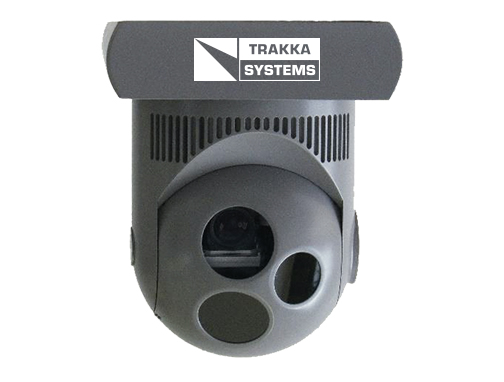
\includegraphics[width=\linewidth]{imagenes/200-LE}
\end{minipage}%
\hfill%
\begin{minipage}{0.7\textwidth}
Especificaciones técnicas
	\begin{itemize}
		\item Diámetro: 200 mm
		\item Peso: 8 kg
		\item Requerimientos de potencia: 22-30 VDC, 250 W
	\end{itemize}
\end{minipage}

\subsubsection*{Trakka Systems TC-300}

\noindent\begin{minipage}{0.3\textwidth}% adapt widths of minipages to your needs
	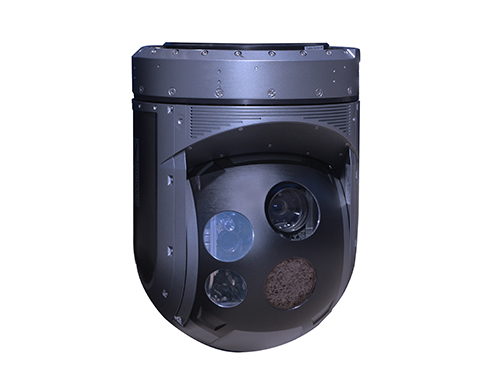
\includegraphics[width=\linewidth]{imagenes/TC-300}
\end{minipage}%
\hfill%
\begin{minipage}{0.7\textwidth}
	Especificaciones técnicas
	\begin{itemize}
		\item Diámetro: 300 mm
		\item Peso: 19 kg
		\item Requerimientos de potencia: 22-36 V, 100-320 W
	\end{itemize}
\end{minipage}

\subsubsection*{Trakka Systems SWE-400 LE}

\noindent\begin{minipage}{0.3\textwidth}% adapt widths of minipages to your needs
	\includegraphics[width=\linewidth]{imagenes/400-le}
\end{minipage}%
\hfill%
\begin{minipage}{0.7\textwidth}
	Especificaciones técnicas
	\begin{itemize}
		\item Diámetro: 400 mm
		\item Peso: 30 kg
		\item Requerimientos de potencia: 22-30VDC, 250 W
	\end{itemize}
\end{minipage}

Estos son solo algunos ejemplos de los sistemas existentes que muestran la enorme variedad de estos, tanto en tamaño y peso como en especificaciones, aunque estas últimas no son objeto de estudio.

Con estos datos se pueden modelizar diferentes cargas que permitan simular diversas condiciones, en el trabajo se emplearán  unas esferas de masa y radio los siguientes:

\begin{itemize}
	\item Carga 1: Masa de 10 kg y radio de 100 mm
	\item Carga 2: Masa de 20 kg y radio de 150 mm
	\item Carga 3: Masa de 30 kg y radio de 200 mm
\end{itemize}

En la tabla \ref{tablaPL} se recogen las características másicas y de inercia de las cargas que han de implementarse en el helicóptero.

\begin{table}[htbp]
	\centering
	\begin{tabular}{|>{\columncolor{Gray}}c|c|}
		\hline
		\cellcolor{Gray}Masa del dispositivo ($M_{pl}$) & 10/20/30 kg \\ \hline
		\cellcolor{Gray}Radio del dispositivo ($R_{pl}$) & 0.1/0.15/0.2 m \\ \hline
		\cellcolor{Gray}Momento de inercia del eje $x$ ($I_{x}^{pl0}$) & 0.04/0.18/0.48 kg$\cdot$m$^2$ \\ \hline
		\cellcolor{Gray}Momento de inercia del eje $y$ ($I_{y}^{pl0}$) & 0.04/0.18/0.48 kg$\cdot$m$^2$ \\ \hline
		\cellcolor{Gray}Momento de inercia del eje $z$ ($I_{z}^{pl0}$) & 0.04/0.18/0.48 kg$\cdot$m$^2$ \\ \hline
		\cellcolor{Gray}Producto de inercia $xy$ ($I_{xy}^{pl0}$)& 0 kg$\cdot$m$^2$ \\ \hline
		\cellcolor{Gray}Producto de inercia $xz$ ($I_{xz}^{pl0}$)& 0 kg$\cdot$m$^2$ \\ \hline
		\cellcolor{Gray}Producto de inercia $yz$ ($I_{yz}^{pl0}$)& 0 kg$\cdot$m$^2$ \\ \hline
		\cellcolor{Gray}Peso del dispositivo ($W_{pl}$)& 10/20/30$\cdot$9.81 N \\ \hline
	\end{tabular}%
	\caption{Valores másicos y de inercia de las diversas cargas de pago que se implementarán en la aeronave.}
	\label{tablaPL}
\end{table}%

\section{Integración de la Carga de Pago}

A la hora de integrar la carga de pago, es muy importante conocer la posición de la misma respecto al centro de masas del helicóptero. Para comprobar que posición puede resultar más favorable, en la tabla \ref{CGPL} se indica un rango de posiciones que se comprobarán en simulaciones posteriores para hallar una posición optima. La posición según el eje $z$ será fija ya que se situará en el suelo del fuselaje en todo momento.

\begin{table}[htbp]
	\centering
	\begin{tabular}{|>{\columncolor{Gray}}c|c|}
		\hline
		\cellcolor{Gray}Posición longitudinal de la carga de pago respecto a $O_f$ ($l_x$) & [-0.65 1.35] m \\ \hline
		\cellcolor{Gray}Posición transversal de la carga de pago respecto a $O_f$ ($l_y$) & [-0.35 0.35] m \\ \hline
		\cellcolor{Gray}Posición vertical del suelo del fuselaje ($l_z$) & 0.6678/0.7178/0.7678 m \\ \hline
	\end{tabular}%
	\caption{Posición de la carga de pago en el fuselaje.}
	\label{CGPL}
\end{table}%

\subsubsection*{Inercia del helicóptero con la carga de pago integrada}

En lo que resta de capítulo, el hiperíndice \emph{$he0$} indicará que se trata de un parámetro del helicóptero en configuración limpia, sin la carga de pago añadida.

Lo primero para poder integrar la carga de pago en la estructura es calcular el nuevo centro de gravedad de la aeronave una vez se ha acoplado la carga de pago. Para ello se pueden usar las siguientes ecuaciones:

\begin{equation}
	X_{CG}^{he}=\frac{x_{CG}^{he0}\cdot W+l_x\cdot W_{pl}}{W+W_{pl}}
\end{equation}
\begin{equation}
	Y_{CG}^{he}=\frac{y_{CG}^{he0}\cdot W+l_y\cdot W_{pl}}{W+W_{pl}}
\end{equation}
\begin{equation}
	Z_{CG}^{he}=\frac{z_{CG}^{he0}\cdot W+l_z\cdot W_{pl}}{W+W_{pl}}
\end{equation}

Una vez posicionado el centro de gravedad del helicóptero, se procede al cálculo de los nuevos valores de inercia de la carga de pago respecto a este centro de masas:

\begin{equation}
I_x^{pl}=I_x^{pl0}+M_{pl}\cdot[(l_y-Y_{CG}^{he})^2+(l_z-Z_{CG}^{he})^2]
\end{equation}
\begin{equation}
I_y^{pl}=I_y^{pl0}+M_{pl}\cdot[(l_x-X_{CG}^{he})^2+(l_z-Z_{CG}^{he})^2]
\end{equation}
\begin{equation}
I_z^{pl}=I_z^{pl0}+M_{pl}\cdot[(l_x-X_{CG}^{he})^2+(l_y-Y_{CG}^{he})^2]
\end{equation}
\begin{equation}
I_x^{pl}=I_x^{pl0}+M_{pl}\cdot(l_y-Y_{CG}^{he})\cdot(l_z-Z_{CG}^{he})
\end{equation}
\begin{equation}
I_y^{pl}=I_y^{pl0}+M_{pl}\cdot(l_x-X_{CG}^{he})\cdot(l_z-Z_{CG}^{he})
\end{equation}
\begin{equation}
I_z^{pl}=I_z^{pl0}+M_{pl}\cdot(l_x-X_{CG}^{he})\cdot(l_y-Y_{CG}^{he})
\end{equation}

El último paso para la integración de la carga de pago consiste en el calculo del tensor de inercia del helicóptero respecto al nuevo centro de gravedad, que se puede calcular con las ecuaciones siguientes:

\begin{equation}
I_x^{he}=I_x^{he0}+M_{pl}\cdot[(y_{CG}^{he0}-Y_{CG}^{he})^2+(z_{CG}^{he0}-Z_{CG}^{he})^2]
\end{equation}
\begin{equation}
I_y^{he}=I_y^{he0}+M_{pl}\cdot[(x_{CG}^{he0}-X_{CG}^{he})^2+(z_{CG}^{he0}-Z_{CG}^{he})^2]
\end{equation}
\begin{equation}
I_z^{he}=I_z^{he0}+M_{pl}\cdot[(x_{CG}^{he0}-X_{CG}^{he})^2+(y_{CG}^{he0}-Y_{CG}^{he})^2]
\end{equation}
\begin{equation}
I_{xy}^{he}=I_{xy}^{he0}+M_{pl}\cdot(x_{CG}^{he0}-X_{CG}^{he})\cdot(y_{CG}^{he0}-Y_{CG}^{he})
\end{equation}
\begin{equation}
I_{xz}^{he}=I_{xx}^{he0}+M_{pl}\cdot(x_{CG}^{he0}-X_{CG}^{he})\cdot(z_{CG}^{he0}-Z_{CG}^{he})
\end{equation}
\begin{equation}
I_{yz}^{he}=I_{yz}^{he0}+M_{pl}\cdot(y_{CG}^{he0}-Y_{CG}^{he})\cdot(z_{CG}^{he0}-Z_{CG}^{he})
\end{equation}

Con estos cálculos ya se han definido todos los parámetros necesarios para poder estudiar el problema del equilibrado del helicóptero con y sin carga de pago, lo que permite realizar las simulaciones de vuelo que se encontrarán en capítulos posteriores de este trabajo.

\singlespacing